% Generated by Sphinx.
\documentclass[a4paper,10pt,english]{manual}
\usepackage[utf8]{inputenc}
\usepackage[T1]{fontenc}
\usepackage{babel}
\usepackage{times}
\usepackage[Bjarne]{fncychap}
\usepackage{longtable}
\usepackage{sphinx}


\title{BIP - Bayesian Inference with Python Documentation}
\date{2010-04-13}
\release{0.4.0}
\author{Flávio Codeço Coelho}
\newcommand{\sphinxlogo}{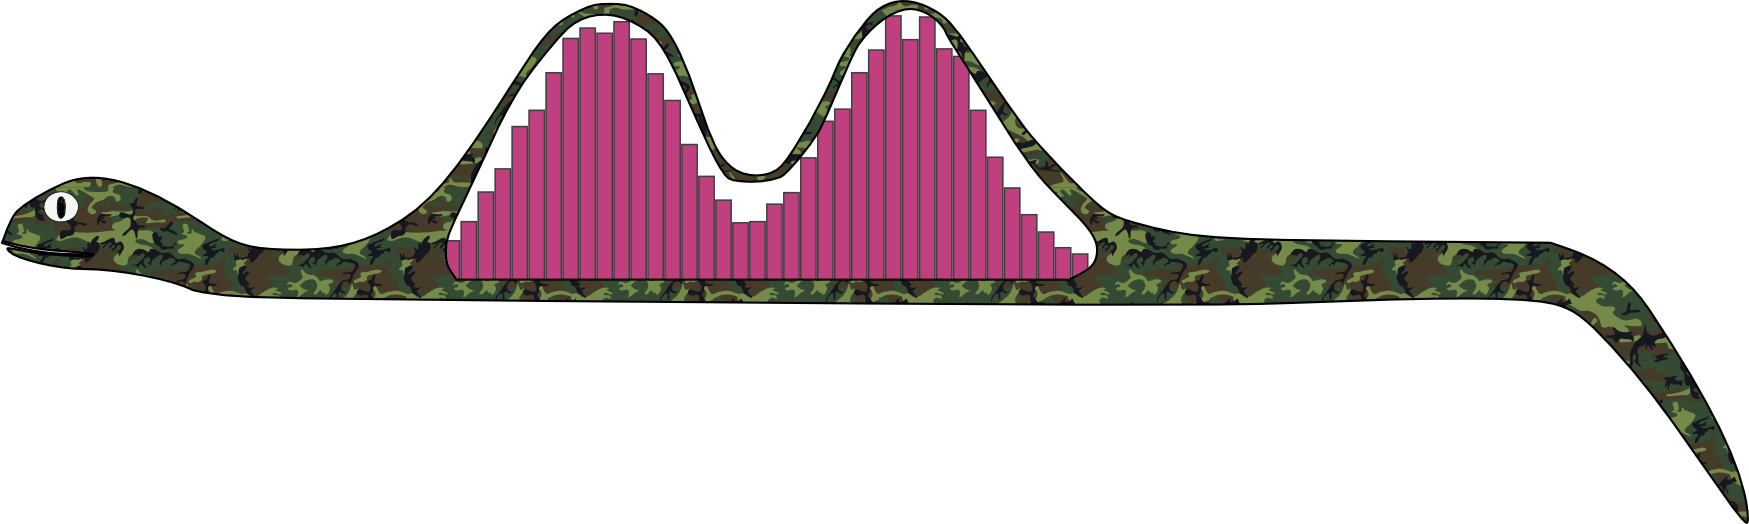
\includegraphics{BIP_large.png}\par}
\renewcommand{\releasename}{Release}
\makeindex
\makemodindex

\makeatletter
\def\PYG@reset{\let\PYG@it=\relax \let\PYG@bf=\relax%
    \let\PYG@ul=\relax \let\PYG@tc=\relax%
    \let\PYG@bc=\relax \let\PYG@ff=\relax}
\def\PYG@tok#1{\csname PYG@tok@#1\endcsname}
\def\PYG@toks#1+{\ifx\relax#1\empty\else%
    \PYG@tok{#1}\expandafter\PYG@toks\fi}
\def\PYG@do#1{\PYG@bc{\PYG@tc{\PYG@ul{%
    \PYG@it{\PYG@bf{\PYG@ff{#1}}}}}}}
\def\PYG#1#2{\PYG@reset\PYG@toks#1+\relax+\PYG@do{#2}}

\def\PYG@tok@gd{\def\PYG@tc##1{\textcolor[rgb]{0.63,0.00,0.00}{##1}}}
\def\PYG@tok@gu{\let\PYG@bf=\textbf\def\PYG@tc##1{\textcolor[rgb]{0.50,0.00,0.50}{##1}}}
\def\PYG@tok@gt{\def\PYG@tc##1{\textcolor[rgb]{0.00,0.25,0.82}{##1}}}
\def\PYG@tok@gs{\let\PYG@bf=\textbf}
\def\PYG@tok@gr{\def\PYG@tc##1{\textcolor[rgb]{1.00,0.00,0.00}{##1}}}
\def\PYG@tok@cm{\let\PYG@it=\textit\def\PYG@tc##1{\textcolor[rgb]{0.25,0.50,0.56}{##1}}}
\def\PYG@tok@vg{\def\PYG@tc##1{\textcolor[rgb]{0.73,0.38,0.84}{##1}}}
\def\PYG@tok@m{\def\PYG@tc##1{\textcolor[rgb]{0.13,0.50,0.31}{##1}}}
\def\PYG@tok@mh{\def\PYG@tc##1{\textcolor[rgb]{0.13,0.50,0.31}{##1}}}
\def\PYG@tok@cs{\def\PYG@tc##1{\textcolor[rgb]{0.25,0.50,0.56}{##1}}\def\PYG@bc##1{\colorbox[rgb]{1.00,0.94,0.94}{##1}}}
\def\PYG@tok@ge{\let\PYG@it=\textit}
\def\PYG@tok@vc{\def\PYG@tc##1{\textcolor[rgb]{0.73,0.38,0.84}{##1}}}
\def\PYG@tok@il{\def\PYG@tc##1{\textcolor[rgb]{0.13,0.50,0.31}{##1}}}
\def\PYG@tok@go{\def\PYG@tc##1{\textcolor[rgb]{0.19,0.19,0.19}{##1}}}
\def\PYG@tok@cp{\def\PYG@tc##1{\textcolor[rgb]{0.00,0.44,0.13}{##1}}}
\def\PYG@tok@gi{\def\PYG@tc##1{\textcolor[rgb]{0.00,0.63,0.00}{##1}}}
\def\PYG@tok@gh{\let\PYG@bf=\textbf\def\PYG@tc##1{\textcolor[rgb]{0.00,0.00,0.50}{##1}}}
\def\PYG@tok@ni{\let\PYG@bf=\textbf\def\PYG@tc##1{\textcolor[rgb]{0.84,0.33,0.22}{##1}}}
\def\PYG@tok@nl{\let\PYG@bf=\textbf\def\PYG@tc##1{\textcolor[rgb]{0.00,0.13,0.44}{##1}}}
\def\PYG@tok@nn{\let\PYG@bf=\textbf\def\PYG@tc##1{\textcolor[rgb]{0.05,0.52,0.71}{##1}}}
\def\PYG@tok@no{\def\PYG@tc##1{\textcolor[rgb]{0.38,0.68,0.84}{##1}}}
\def\PYG@tok@na{\def\PYG@tc##1{\textcolor[rgb]{0.25,0.44,0.63}{##1}}}
\def\PYG@tok@nb{\def\PYG@tc##1{\textcolor[rgb]{0.00,0.44,0.13}{##1}}}
\def\PYG@tok@nc{\let\PYG@bf=\textbf\def\PYG@tc##1{\textcolor[rgb]{0.05,0.52,0.71}{##1}}}
\def\PYG@tok@nd{\let\PYG@bf=\textbf\def\PYG@tc##1{\textcolor[rgb]{0.33,0.33,0.33}{##1}}}
\def\PYG@tok@ne{\def\PYG@tc##1{\textcolor[rgb]{0.00,0.44,0.13}{##1}}}
\def\PYG@tok@nf{\def\PYG@tc##1{\textcolor[rgb]{0.02,0.16,0.49}{##1}}}
\def\PYG@tok@si{\let\PYG@it=\textit\def\PYG@tc##1{\textcolor[rgb]{0.44,0.63,0.82}{##1}}}
\def\PYG@tok@s2{\def\PYG@tc##1{\textcolor[rgb]{0.25,0.44,0.63}{##1}}}
\def\PYG@tok@vi{\def\PYG@tc##1{\textcolor[rgb]{0.73,0.38,0.84}{##1}}}
\def\PYG@tok@nt{\let\PYG@bf=\textbf\def\PYG@tc##1{\textcolor[rgb]{0.02,0.16,0.45}{##1}}}
\def\PYG@tok@nv{\def\PYG@tc##1{\textcolor[rgb]{0.73,0.38,0.84}{##1}}}
\def\PYG@tok@s1{\def\PYG@tc##1{\textcolor[rgb]{0.25,0.44,0.63}{##1}}}
\def\PYG@tok@gp{\let\PYG@bf=\textbf\def\PYG@tc##1{\textcolor[rgb]{0.78,0.36,0.04}{##1}}}
\def\PYG@tok@sh{\def\PYG@tc##1{\textcolor[rgb]{0.25,0.44,0.63}{##1}}}
\def\PYG@tok@ow{\let\PYG@bf=\textbf\def\PYG@tc##1{\textcolor[rgb]{0.00,0.44,0.13}{##1}}}
\def\PYG@tok@sx{\def\PYG@tc##1{\textcolor[rgb]{0.78,0.36,0.04}{##1}}}
\def\PYG@tok@bp{\def\PYG@tc##1{\textcolor[rgb]{0.00,0.44,0.13}{##1}}}
\def\PYG@tok@c1{\let\PYG@it=\textit\def\PYG@tc##1{\textcolor[rgb]{0.25,0.50,0.56}{##1}}}
\def\PYG@tok@kc{\let\PYG@bf=\textbf\def\PYG@tc##1{\textcolor[rgb]{0.00,0.44,0.13}{##1}}}
\def\PYG@tok@c{\let\PYG@it=\textit\def\PYG@tc##1{\textcolor[rgb]{0.25,0.50,0.56}{##1}}}
\def\PYG@tok@mf{\def\PYG@tc##1{\textcolor[rgb]{0.13,0.50,0.31}{##1}}}
\def\PYG@tok@err{\def\PYG@bc##1{\fcolorbox[rgb]{1.00,0.00,0.00}{1,1,1}{##1}}}
\def\PYG@tok@kd{\let\PYG@bf=\textbf\def\PYG@tc##1{\textcolor[rgb]{0.00,0.44,0.13}{##1}}}
\def\PYG@tok@ss{\def\PYG@tc##1{\textcolor[rgb]{0.32,0.47,0.09}{##1}}}
\def\PYG@tok@sr{\def\PYG@tc##1{\textcolor[rgb]{0.14,0.33,0.53}{##1}}}
\def\PYG@tok@mo{\def\PYG@tc##1{\textcolor[rgb]{0.13,0.50,0.31}{##1}}}
\def\PYG@tok@mi{\def\PYG@tc##1{\textcolor[rgb]{0.13,0.50,0.31}{##1}}}
\def\PYG@tok@kn{\let\PYG@bf=\textbf\def\PYG@tc##1{\textcolor[rgb]{0.00,0.44,0.13}{##1}}}
\def\PYG@tok@o{\def\PYG@tc##1{\textcolor[rgb]{0.40,0.40,0.40}{##1}}}
\def\PYG@tok@kr{\let\PYG@bf=\textbf\def\PYG@tc##1{\textcolor[rgb]{0.00,0.44,0.13}{##1}}}
\def\PYG@tok@s{\def\PYG@tc##1{\textcolor[rgb]{0.25,0.44,0.63}{##1}}}
\def\PYG@tok@kp{\def\PYG@tc##1{\textcolor[rgb]{0.00,0.44,0.13}{##1}}}
\def\PYG@tok@w{\def\PYG@tc##1{\textcolor[rgb]{0.73,0.73,0.73}{##1}}}
\def\PYG@tok@kt{\def\PYG@tc##1{\textcolor[rgb]{0.56,0.13,0.00}{##1}}}
\def\PYG@tok@sc{\def\PYG@tc##1{\textcolor[rgb]{0.25,0.44,0.63}{##1}}}
\def\PYG@tok@sb{\def\PYG@tc##1{\textcolor[rgb]{0.25,0.44,0.63}{##1}}}
\def\PYG@tok@k{\let\PYG@bf=\textbf\def\PYG@tc##1{\textcolor[rgb]{0.00,0.44,0.13}{##1}}}
\def\PYG@tok@se{\let\PYG@bf=\textbf\def\PYG@tc##1{\textcolor[rgb]{0.25,0.44,0.63}{##1}}}
\def\PYG@tok@sd{\let\PYG@it=\textit\def\PYG@tc##1{\textcolor[rgb]{0.25,0.44,0.63}{##1}}}

\def\PYGZat{@}
\def\PYGZlb{[}
\def\PYGZrb{]}
\makeatother

\begin{document}

\maketitle
\tableofcontents
\hypertarget{--doc-index}{}


This documentation corresponds to version 0.4.0.


\chapter{Contents}

\resetcurrentobjects
\hypertarget{--doc-overview}{}

\section{Overview}

The Bip Package is a collection of useful classes for basic Bayesian inference. Currently, its main goal is to be a tool for learning and exploration of Bayesian probabilistic calculations.

Currently it also includes subpackages for stochastic simulation tools which are not strictly related to Bayesian inference, but are currently being developed within BIP. One such package is the BIP.SDE which contains a parallelized solver for stochastic differential equations, an implementation of the Gillespie direct algorithm.

The Subpackage Bayes also offers a tool for parameter estimation of Deterministic and Stochastic Dynamical Models. This tool will be fully described briefly in a scientific paper currently submitted for publication.

\resetcurrentobjects
\hypertarget{--doc-paramest}{}

\section{Parameter Estimation in Dynamic Models}

A growing theme in mathematical modeling is uncertainty analysis. The Melding Module provides a Bayesian framework to analyze uncertainty in mathematical models. It includes tools that allow modellers to integrate Prior information about the model's parameters and variables into the model, in order to explore the full uncertainty associated with a model.

This framework is inspired on the original Bayesian Melding paper by Poole and Raftery \footnote{
Poole, D., \& Raftery, A. E. (2000). Inference for Deterministic Simulation Models: The Bayesian Melding Approach. Journal of the American Statistical Association, 95(452), 1244-1255. doi:10.2307/2669764
}, but extended to handle dynamical systems and different posterior sampling mechanisms, i.e., the user has the choice to use Sampling Importance resampling, Approximate Bayesian computations or MCMC.

Once a model is thus parameterized, we can simulate the model, with full uncertainty representation and also fit the model to available data to reduce that uncertaity. Markov chain Monte Carlo algorithms are at the core of the framework, which requires a large number of simulations of the models in order to explore parameter space.


\subsection{Single Session Retrospective estimation}

Frequently, we have a complete time series corresponding to one or more state variables of our dynamic model. In such cases it may be interesting to use this information, to estimate the parameter values which maximize the fit of our model to the data. Below are examples of such inference situations.


\subsubsection{Example Usage}

This first example includes a simple ODE (an SIR epidemic model) model which is fitted against simulated data to which noise is added:

\begin{Verbatim}[commandchars=@\[\]]
@PYG[c][@#-*- coding: utf-8 -*-]
@PYG[l+s+sd]["""]
@PYG[l+s+sd][Parameter estimation and series forcasting based on simulated data with moving window.]
@PYG[l+s+sd][Deterministic model]
@PYG[l+s+sd]["""]
@PYG[c][@#]
@PYG[c][@# Copyright 2009- by Flávio Codeço Coelho]
@PYG[c][@# License gpl v3]
@PYG[c][@#]
@PYG[k+kn][from] @PYG[n+nn][BIP.Bayes.Melding] @PYG[k+kn][import] @PYG[n][FitModel]
@PYG[k+kn][from] @PYG[n+nn][scipy.integrate] @PYG[k+kn][import] @PYG[n][odeint]
@PYG[k+kn][import] @PYG[n+nn][scipy.stats] @PYG[k+kn][as] @PYG[n+nn][st]
@PYG[k+kn][import] @PYG[n+nn][numpy] @PYG[k+kn][as] @PYG[n+nn][np]

@PYG[n][beta] @PYG[o][=] @PYG[l+m+mi][1] @PYG[c][@#Transmission coefficient]
@PYG[n][tau] @PYG[o][=] @PYG[o][.]@PYG[l+m+mi][2] @PYG[c][@#infectious period. FIXED]
@PYG[n][tf] @PYG[o][=] @PYG[l+m+mi][36]
@PYG[n][y0] @PYG[o][=] @PYG[p][@PYGZlb[]]@PYG[o][.]@PYG[l+m+mi][999]@PYG[p][,]@PYG[l+m+mf][0.001]@PYG[p][,]@PYG[l+m+mf][0.0]@PYG[p][@PYGZrb[]]
@PYG[k][def] @PYG[n+nf][model]@PYG[p][(]@PYG[n][theta]@PYG[p][)]@PYG[p][:]
    @PYG[n][beta] @PYG[o][=] @PYG[n][theta]@PYG[p][@PYGZlb[]]@PYG[l+m+mi][0]@PYG[p][@PYGZrb[]]
    @PYG[k][def] @PYG[n+nf][sir]@PYG[p][(]@PYG[n][y]@PYG[p][,]@PYG[n][t]@PYG[p][)]@PYG[p][:]
        @PYG[l+s+sd]['''ODE model''']
        @PYG[n][S]@PYG[p][,]@PYG[n][I]@PYG[p][,]@PYG[n][R] @PYG[o][=] @PYG[n][y]
        @PYG[k][return]  @PYG[p][@PYGZlb[]]@PYG[o][-]@PYG[n][beta]@PYG[o][*]@PYG[n][I]@PYG[o][*]@PYG[n][S]@PYG[p][,] @PYG[c][@#dS/dt]
                @PYG[n][beta]@PYG[o][*]@PYG[n][I]@PYG[o][*]@PYG[n][S] @PYG[o][-] @PYG[n][tau]@PYG[o][*]@PYG[n][I]@PYG[p][,] @PYG[c][@#dI/dt]
                @PYG[n][tau]@PYG[o][*]@PYG[n][I]@PYG[p][@PYGZrb[]] @PYG[c][@#dR/dt]
    @PYG[n][y] @PYG[o][=] @PYG[n][odeint]@PYG[p][(]@PYG[n][sir]@PYG[p][,]@PYG[n][inits]@PYG[p][,]@PYG[n][np]@PYG[o][.]@PYG[n][arange]@PYG[p][(]@PYG[l+m+mi][0]@PYG[p][,]@PYG[n][tf]@PYG[p][,]@PYG[l+m+mi][1]@PYG[p][)]@PYG[p][)]@PYG[c][@#np.arange(t0,tf,step))]
    @PYG[k][return] @PYG[n][y]
    
@PYG[n][F] @PYG[o][=] @PYG[n][FitModel]@PYG[p][(]@PYG[l+m+mi][300]@PYG[p][,] @PYG[n][model]@PYG[p][,]@PYG[n][y0]@PYG[p][,]@PYG[n][tf]@PYG[p][,]@PYG[p][@PYGZlb[]]@PYG[l+s][']@PYG[l+s][beta]@PYG[l+s][']@PYG[p][@PYGZrb[]]@PYG[p][,]@PYG[p][@PYGZlb[]]@PYG[l+s][']@PYG[l+s][S]@PYG[l+s][']@PYG[p][,]@PYG[l+s][']@PYG[l+s][I]@PYG[l+s][']@PYG[p][,]@PYG[l+s][']@PYG[l+s][R]@PYG[l+s][']@PYG[p][@PYGZrb[]]@PYG[p][,]
            @PYG[n][wl]@PYG[o][=]@PYG[l+m+mi][36]@PYG[p][,]@PYG[n][nw]@PYG[o][=]@PYG[l+m+mi][1]@PYG[p][,]@PYG[n][verbose]@PYG[o][=]@PYG[l+m+mi][1]@PYG[p][,]@PYG[n][burnin]@PYG[o][=]@PYG[l+m+mi][100]@PYG[p][)]
@PYG[n][F]@PYG[o][.]@PYG[n][set@_priors]@PYG[p][(]@PYG[n][tdists]@PYG[o][=]@PYG[p][@PYGZlb[]]@PYG[n][st]@PYG[o][.]@PYG[n][norm]@PYG[p][@PYGZrb[]]@PYG[p][,]@PYG[n][tpars]@PYG[o][=]@PYG[p][@PYGZlb[]]@PYG[p][(]@PYG[l+m+mf][1.1]@PYG[p][,]@PYG[o][.]@PYG[l+m+mi][2]@PYG[p][)]@PYG[p][@PYGZrb[]]@PYG[p][,]@PYG[n][tlims]@PYG[o][=]@PYG[p][@PYGZlb[]]@PYG[p][(]@PYG[l+m+mf][0.5]@PYG[p][,]@PYG[l+m+mf][1.5]@PYG[p][)]@PYG[p][@PYGZrb[]]@PYG[p][,]
    @PYG[n][pdists]@PYG[o][=]@PYG[p][@PYGZlb[]]@PYG[n][st]@PYG[o][.]@PYG[n][uniform]@PYG[p][@PYGZrb[]]@PYG[o][*]@PYG[l+m+mi][3]@PYG[p][,]@PYG[n][ppars]@PYG[o][=]@PYG[p][@PYGZlb[]]@PYG[p][(]@PYG[l+m+mi][0]@PYG[p][,]@PYG[o][.]@PYG[l+m+mi][1]@PYG[p][)]@PYG[p][,]@PYG[p][(]@PYG[l+m+mi][0]@PYG[p][,]@PYG[o][.]@PYG[l+m+mi][1]@PYG[p][)]@PYG[p][,]@PYG[p][(]@PYG[o][.]@PYG[l+m+mi][8]@PYG[p][,]@PYG[o][.]@PYG[l+m+mi][2]@PYG[p][)]@PYG[p][@PYGZrb[]]@PYG[p][,]@PYG[n][plims]@PYG[o][=]@PYG[p][@PYGZlb[]]@PYG[p][(]@PYG[l+m+mi][0]@PYG[p][,]@PYG[l+m+mi][1]@PYG[p][)]@PYG[p][@PYGZrb[]]@PYG[o][*]@PYG[l+m+mi][3]@PYG[p][)]
@PYG[n][d] @PYG[o][=] @PYG[n][model]@PYG[p][(]@PYG[p][@PYGZlb[]]@PYG[l+m+mf][1.0]@PYG[p][@PYGZrb[]]@PYG[p][)] @PYG[c][@#simulate some data]
@PYG[n][noise] @PYG[o][=] @PYG[n][st]@PYG[o][.]@PYG[n][norm]@PYG[p][(]@PYG[l+m+mi][0]@PYG[p][,]@PYG[l+m+mf][0.01]@PYG[p][)]@PYG[o][.]@PYG[n][rvs]@PYG[p][(]@PYG[l+m+mi][36]@PYG[p][)]
@PYG[n][dt] @PYG[o][=] @PYG[p][{]@PYG[l+s][']@PYG[l+s][I]@PYG[l+s][']@PYG[p][:]@PYG[n][d]@PYG[p][@PYGZlb[]]@PYG[p][:]@PYG[p][,]@PYG[l+m+mi][1]@PYG[p][@PYGZrb[]]@PYG[o][+]@PYG[n][noise]@PYG[p][}] @PYG[c][@# add noise]
@PYG[n][F]@PYG[o][.]@PYG[n][run]@PYG[p][(]@PYG[n][dt]@PYG[p][,]@PYG[l+s][']@PYG[l+s][MCMC]@PYG[l+s][']@PYG[p][,]@PYG[n][likvar]@PYG[o][=]@PYG[l+m+mf][1e-4]@PYG[p][,]@PYG[n][pool]@PYG[o][=]@PYG[n+nb+bp][True]@PYG[p][,]@PYG[n][monitor]@PYG[o][=]@PYG[p][@PYGZlb[]]@PYG[p][@PYGZrb[]]@PYG[p][)]
@PYG[c][@#==Uncomment the line below to see plots of the results]
@PYG[n][F]@PYG[o][.]@PYG[n][plot@_results]@PYG[p][(]@PYG[p][)]
\end{Verbatim}

The code above starts by defining the models parameters and initial conditions, and a function which takes in the parameters runs the model and returns the output.

After that, we Instantiate our fitting Object:

\begin{Verbatim}[commandchars=@\[\]]
@PYG[n][F] @PYG[o][=] @PYG[n][FitModel]@PYG[p][(]@PYG[l+m+mi][300]@PYG[p][,]@PYG[n][model]@PYG[p][,]@PYG[n][y0]@PYG[p][,]@PYG[n][tf]@PYG[p][,]@PYG[p][@PYGZlb[]]@PYG[l+s][']@PYG[l+s][beta]@PYG[l+s][']@PYG[p][@PYGZrb[]]@PYG[p][,]@PYG[p][@PYGZlb[]]@PYG[l+s][']@PYG[l+s][S]@PYG[l+s][']@PYG[p][,]@PYG[l+s][']@PYG[l+s][I]@PYG[l+s][']@PYG[p][,]@PYG[l+s][']@PYG[l+s][R]@PYG[l+s][']@PYG[p][@PYGZrb[]]@PYG[p][,]
            @PYG[n][wl]@PYG[o][=]@PYG[l+m+mi][36]@PYG[p][,]@PYG[n][nw]@PYG[o][=]@PYG[l+m+mi][1]@PYG[p][,]@PYG[n][verbose]@PYG[o][=]@PYG[n+nb+bp][False]@PYG[p][,]@PYG[n][burnin]@PYG[o][=]@PYG[l+m+mi][100]@PYG[p][)]
\end{Verbatim}

Here we have to pass a few arguments: the first (\code{K=300}) is the number of samples we will take from the joint prior distribution of the parameters to run the inference. The second one (\code{model}) is the callable(function) which corresponds to the model you want to fit to data. Then you have the initial condition vector(\code{inits=y0}), the list of parameter names (\code{thetanames = {[}'beta'{]}}), the list of variable names (\code{phinames={[}'S','I','R'{]}}), inference window length (\code{wl=36}), number of juxtaposed windows (\code{nw=1}), verbosity flag (\code{verbose=False}) and finally the number of burnin samples (\code{burnin=1000}), which is only needed for if the inference method chosen is \code{MCMC}.

One should always have \code{verbose=True} on a first fitting run of a model or if the simulations seems to be taking longer than expected. When \code{verbose} is true, printed and graphical is generated regarding the behavior of fitting, which can be useful to fine tune its parameters.

The next line of code also carries a lot of relevant information about the inference: the specification of the prior distributions. By now you must have noticed that not all parameters included in the model need to be included in the analysis. any number of them except for one can be set constant, which is what happens with the parameter \code{tau} in this example:

\begin{Verbatim}[commandchars=@\[\]]
@PYG[n][F]@PYG[o][.]@PYG[n][set@_priors]@PYG[p][(]@PYG[n][tdists]@PYG[o][=]@PYG[p][@PYGZlb[]]@PYG[n][st]@PYG[o][.]@PYG[n][norm]@PYG[p][@PYGZrb[]]@PYG[p][,]@PYG[n][tpars]@PYG[o][=]@PYG[p][@PYGZlb[]]@PYG[p][(]@PYG[l+m+mf][1.1]@PYG[p][,]@PYG[o][.]@PYG[l+m+mi][2]@PYG[p][)]@PYG[p][@PYGZrb[]]@PYG[p][,]@PYG[n][tlims]@PYG[o][=]@PYG[p][@PYGZlb[]]@PYG[p][(]@PYG[l+m+mf][0.5]@PYG[p][,]@PYG[l+m+mf][1.5]@PYG[p][)]@PYG[p][@PYGZrb[]]@PYG[p][,]
    @PYG[n][pdists]@PYG[o][=]@PYG[p][@PYGZlb[]]@PYG[n][st]@PYG[o][.]@PYG[n][uniform]@PYG[p][@PYGZrb[]]@PYG[o][*]@PYG[l+m+mi][3]@PYG[p][,]@PYG[n][ppars]@PYG[o][=]@PYG[p][@PYGZlb[]]@PYG[p][(]@PYG[l+m+mi][0]@PYG[p][,]@PYG[o][.]@PYG[l+m+mi][1]@PYG[p][)]@PYG[p][,]@PYG[p][(]@PYG[l+m+mi][0]@PYG[p][,]@PYG[o][.]@PYG[l+m+mi][1]@PYG[p][)]@PYG[p][,]@PYG[p][(]@PYG[o][.]@PYG[l+m+mi][8]@PYG[p][,]@PYG[o][.]@PYG[l+m+mi][2]@PYG[p][)]@PYG[p][@PYGZrb[]]@PYG[p][,]@PYG[n][plims]@PYG[o][=]@PYG[p][@PYGZlb[]]@PYG[p][(]@PYG[l+m+mi][0]@PYG[p][,]@PYG[l+m+mi][1]@PYG[p][)]@PYG[p][@PYGZrb[]]@PYG[o][*]@PYG[l+m+mi][3]@PYG[p][)]
\end{Verbatim}

here we set the prior distributions for the theta (the model's parameters) and phi (the model's variables). \code{tdists}, \code{tpars} and \code{tlims} are theta's distributions, parameters, and ranges. For example here we use a Normal distribution (\code{st.norm}) for \code{beta}, with mean and standard deviation equal to 1.1 and .2, respectively. we also set the range of \code{beta} to be from 0.5 to 1.5. We do the same for phi.

The remaining lines just generate some simulated data to fit the model with, run the inference and plot the results which should include plots like this:
\begin{figure}[htbp]
\centering

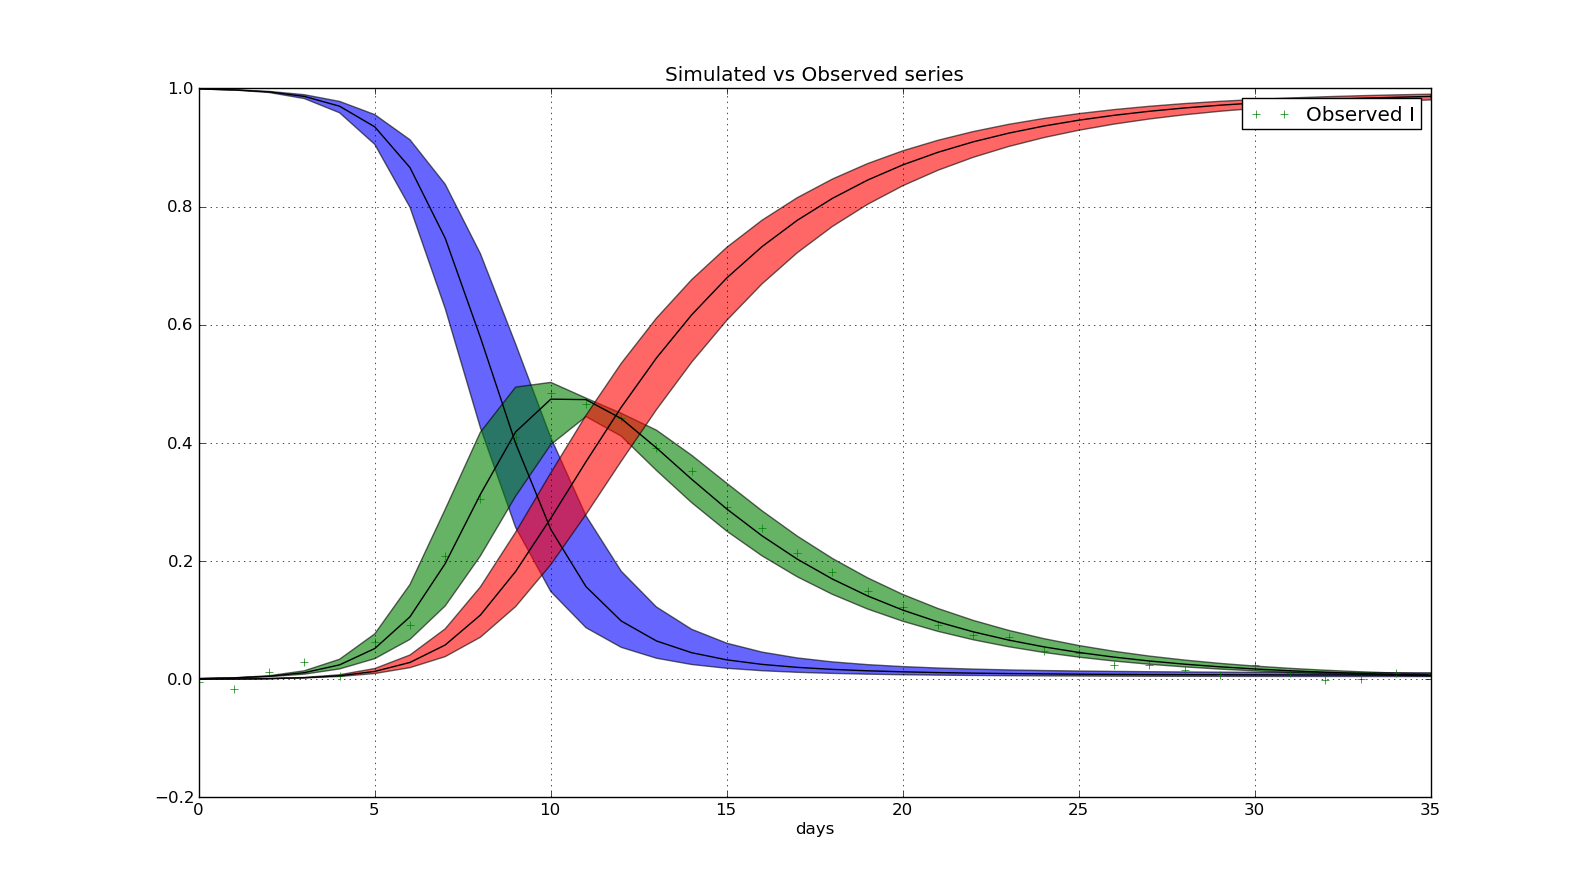
\includegraphics[width=15cm]{fit_series.png}
\caption{Series posterior distributions. Colored areas represent 95\% credible intervals.}\end{figure}
\begin{figure}[htbp]
\centering

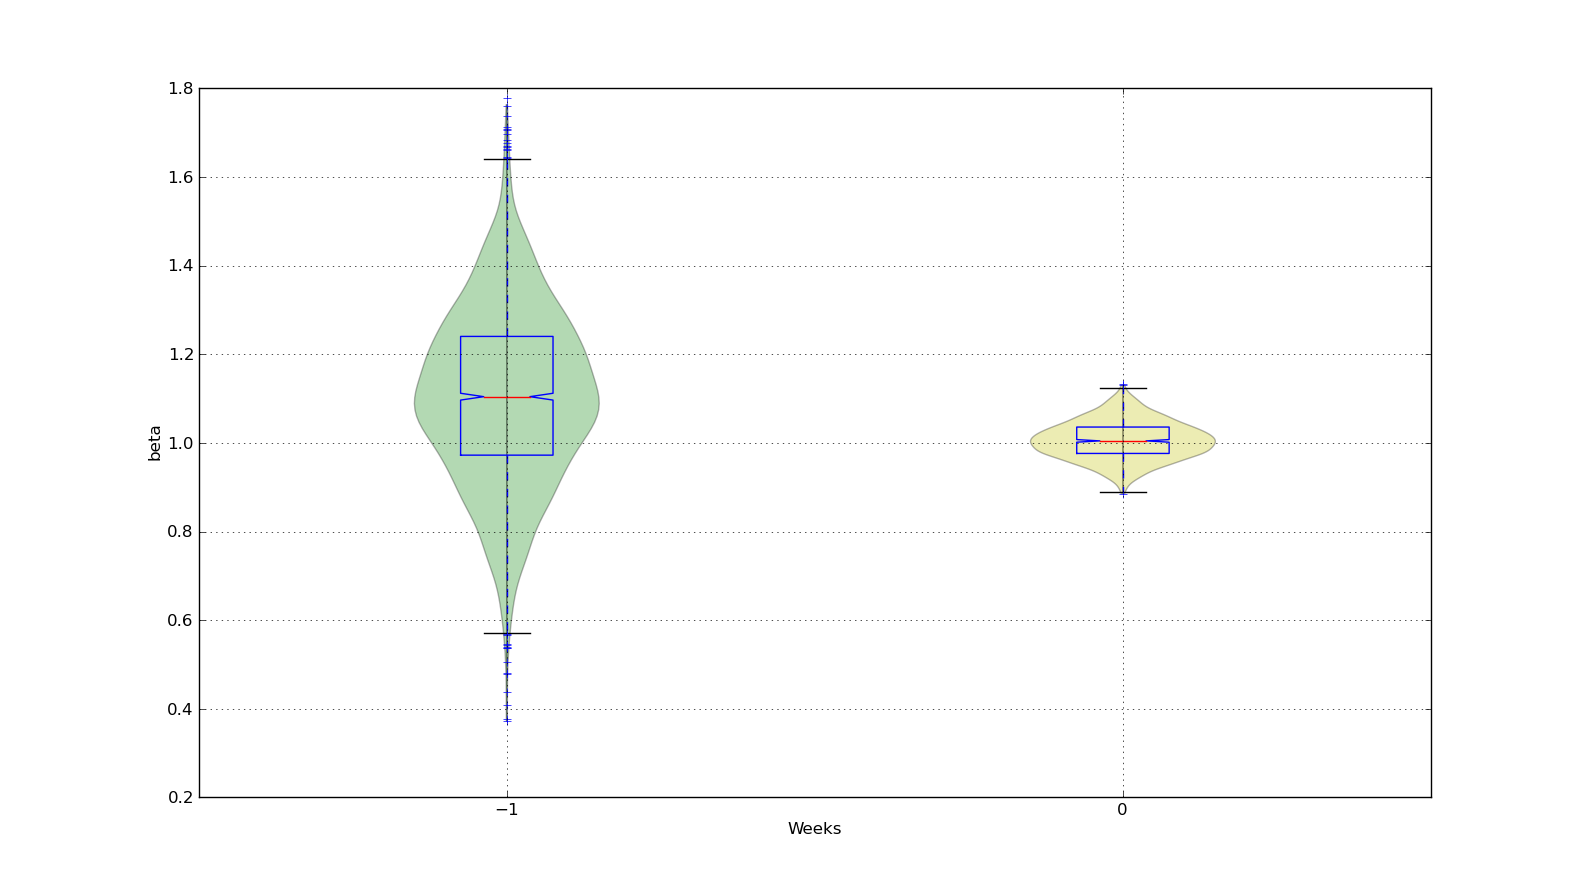
\includegraphics[width=15cm]{fit_par.png}
\end{figure}

One important argument in the run call, is the likvar, Which is the initial value for the likelihood variance. Try to increase its value if the acceptance ratio of the markov chain is too llow. Ideal levels for the acceptance ratio should be between 0.3 and 0.5.

The code for the above example can be found in the examples directory of the BIP distribution as \textbf{deterministic.py}


\subsubsection{Stochastic Model Example}

This example fits a stochastic model to simulated data. It uses the \hyperlink{sde}{\emph{SDE}} package of BIP:

\begin{Verbatim}[commandchars=@\[\]]
@PYG[c][@#-*- coding:utf-8 -*-]
@PYG[l+s+sd]["""]
@PYG[l+s+sd][Parameter estimation and series forcasting based on simulated data with moving window.]
@PYG[l+s+sd][Stochastic model]
@PYG[l+s+sd]["""]
@PYG[c][@#]
@PYG[c][@# Copyright 2009- by Flávio Codeço Coelho]
@PYG[c][@# License gpl v3]
@PYG[c][@#]
@PYG[k+kn][from] @PYG[n+nn][BIP.SDE.gillespie] @PYG[k+kn][import] @PYG[n][Model]
@PYG[k+kn][from] @PYG[n+nn][BIP.Bayes.Melding] @PYG[k+kn][import] @PYG[n][FitModel]
@PYG[k+kn][import] @PYG[n+nn][numpy] @PYG[k+kn][as] @PYG[n+nn][np]
@PYG[k+kn][from] @PYG[n+nn][scipy] @PYG[k+kn][import] @PYG[n][stats] @PYG[k][as] @PYG[n][st]

@PYG[n][mu] @PYG[o][=] @PYG[l+m+mf][0.0] @PYG[c][@#birth and death rate.FIXED]
@PYG[n][beta] @PYG[o][=] @PYG[l+m+mf][0.00058] @PYG[c][@#Transmission rate]
@PYG[n][eta] @PYG[o][=] @PYG[o][.]@PYG[l+m+mi][5] @PYG[c][@#infectivity of asymptomatic infections relative to clinical ones. FIXED]
@PYG[n][epsilon] @PYG[o][=] @PYG[o][.]@PYG[l+m+mi][1] @PYG[c][@#latency period ]
@PYG[n][alpha] @PYG[o][=] @PYG[o][.]@PYG[l+m+mi][2] @PYG[c][@#Probability of developing clinical influenza symptoms]
@PYG[n][sigma] @PYG[o][=] @PYG[o][.]@PYG[l+m+mi][5] @PYG[c][@#reduced risk of re-infection after recovery]
@PYG[n][tau] @PYG[o][=] @PYG[o][.]@PYG[l+m+mo][01] @PYG[c][@#infectious period. FIXED]
@PYG[c][@# Initial conditions]
@PYG[k][global] @PYG[n][inits]@PYG[p][,]@PYG[n][tf]
@PYG[n][tf]@PYG[o][=] @PYG[l+m+mi][140]
@PYG[n][inits] @PYG[o][=] @PYG[p][@PYGZlb[]]@PYG[l+m+mi][490]@PYG[p][,]@PYG[l+m+mi][0]@PYG[p][,]@PYG[l+m+mi][10]@PYG[p][,]@PYG[l+m+mi][0]@PYG[p][,]@PYG[l+m+mi][0]@PYG[p][@PYGZrb[]]
@PYG[n][pars] @PYG[o][=] @PYG[p][@PYGZlb[]]@PYG[n][beta]@PYG[p][,]@PYG[n][alpha]@PYG[p][,]@PYG[n][sigma]@PYG[p][@PYGZrb[]]


@PYG[c][@# propensity functions]
@PYG[k][def] @PYG[n+nf][f1]@PYG[p][(]@PYG[n][r]@PYG[p][,]@PYG[n][inits]@PYG[p][)]@PYG[p][:]@PYG[k][return] @PYG[n][r]@PYG[p][@PYGZlb[]]@PYG[l+m+mi][0]@PYG[p][@PYGZrb[]]@PYG[o][*]@PYG[n][inits]@PYG[p][@PYGZlb[]]@PYG[l+m+mi][0]@PYG[p][@PYGZrb[]]@PYG[o][*]@PYG[p][(]@PYG[n][inits]@PYG[p][@PYGZlb[]]@PYG[l+m+mi][2]@PYG[p][@PYGZrb[]]@PYG[o][+]@PYG[n][inits]@PYG[p][@PYGZlb[]]@PYG[l+m+mi][3]@PYG[p][@PYGZrb[]]@PYG[p][)]@PYG[c][@#S-@textgreater[]E]
@PYG[k][def] @PYG[n+nf][f2]@PYG[p][(]@PYG[n][r]@PYG[p][,]@PYG[n][inits]@PYG[p][)]@PYG[p][:]@PYG[k][return] @PYG[n][r]@PYG[p][@PYGZlb[]]@PYG[l+m+mi][1]@PYG[p][@PYGZrb[]]@PYG[o][*]@PYG[n][inits]@PYG[p][@PYGZlb[]]@PYG[l+m+mi][1]@PYG[p][@PYGZrb[]]@PYG[c][@#E-@textgreater[]I]
@PYG[k][def] @PYG[n+nf][f3]@PYG[p][(]@PYG[n][r]@PYG[p][,]@PYG[n][inits]@PYG[p][)]@PYG[p][:]@PYG[k][return] @PYG[n][r]@PYG[p][@PYGZlb[]]@PYG[l+m+mi][3]@PYG[p][@PYGZrb[]]@PYG[o][*]@PYG[n][inits]@PYG[p][@PYGZlb[]]@PYG[l+m+mi][2]@PYG[p][@PYGZrb[]]@PYG[c][@#I-@textgreater[]R]
@PYG[k][def] @PYG[n+nf][f4]@PYG[p][(]@PYG[n][r]@PYG[p][,]@PYG[n][inits]@PYG[p][)]@PYG[p][:]@PYG[k][return] @PYG[n][r]@PYG[p][@PYGZlb[]]@PYG[l+m+mi][2]@PYG[p][@PYGZrb[]]@PYG[o][*]@PYG[n][inits]@PYG[p][@PYGZlb[]]@PYG[l+m+mi][1]@PYG[p][@PYGZrb[]]@PYG[c][@#E-@textgreater[]A]
@PYG[k][def] @PYG[n+nf][f5]@PYG[p][(]@PYG[n][r]@PYG[p][,]@PYG[n][inits]@PYG[p][)]@PYG[p][:]@PYG[k][return] @PYG[n][r]@PYG[p][@PYGZlb[]]@PYG[l+m+mi][4]@PYG[p][@PYGZrb[]]@PYG[o][*]@PYG[n][inits]@PYG[p][@PYGZlb[]]@PYG[l+m+mi][3]@PYG[p][@PYGZrb[]]@PYG[c][@#A-@textgreater[]R]

@PYG[k][def] @PYG[n+nf][runModel]@PYG[p][(]@PYG[n][theta]@PYG[p][)]@PYG[p][:]
    @PYG[k][global] @PYG[n][tf]@PYG[p][,]@PYG[n][inits]
    @PYG[n][step] @PYG[o][=] @PYG[l+m+mi][1]
    @PYG[c][@#setting parameters]
    @PYG[n][beta]@PYG[p][,]@PYG[n][alpha]@PYG[p][,]@PYG[n][sigma] @PYG[o][=] @PYG[n][theta]@PYG[p][@PYGZlb[]]@PYG[p][:]@PYG[l+m+mi][3]@PYG[p][@PYGZrb[]]
    @PYG[n][vnames] @PYG[o][=] @PYG[p][@PYGZlb[]]@PYG[l+s][']@PYG[l+s][S]@PYG[l+s][']@PYG[p][,]@PYG[l+s][']@PYG[l+s][E]@PYG[l+s][']@PYG[p][,]@PYG[l+s][']@PYG[l+s][I]@PYG[l+s][']@PYG[p][,]@PYG[l+s][']@PYG[l+s][A]@PYG[l+s][']@PYG[p][,]@PYG[l+s][']@PYG[l+s][R]@PYG[l+s][']@PYG[p][@PYGZrb[]]
    @PYG[c][@#rates: b,ki,ka,ri,ra]
    @PYG[c][@#r = (0.001, 0.1, 0.1, 0.01, 0.01)]
    @PYG[n][r] @PYG[o][=] @PYG[p][(]@PYG[n][beta]@PYG[p][,] @PYG[p][(]@PYG[n][alpha]@PYG[p][)]@PYG[o][*]@PYG[n][epsilon]@PYG[p][,] @PYG[p][(]@PYG[l+m+mi][1]@PYG[o][-]@PYG[n][alpha]@PYG[p][)]@PYG[o][*]@PYG[n][epsilon]@PYG[p][,] @PYG[n][tau]@PYG[p][,] @PYG[n][tau]@PYG[p][)]
    @PYG[c][@#print r,inits]
    @PYG[c][@# propensity functions]
    @PYG[n][propf] @PYG[o][=] @PYG[p][(]@PYG[n][f1]@PYG[p][,]@PYG[n][f2]@PYG[p][,]@PYG[n][f3]@PYG[p][,]@PYG[n][f4]@PYG[p][,]@PYG[n][f5]@PYG[p][)]

    @PYG[n][tmat] @PYG[o][=] @PYG[n][np]@PYG[o][.]@PYG[n][array]@PYG[p][(]@PYG[p][@PYGZlb[]]@PYG[p][@PYGZlb[]]@PYG[o][-]@PYG[l+m+mi][1]@PYG[p][,] @PYG[l+m+mi][0]@PYG[p][,] @PYG[l+m+mi][0]@PYG[p][,] @PYG[l+m+mi][0]@PYG[p][,] @PYG[l+m+mi][0]@PYG[p][@PYGZrb[]]@PYG[p][,]
                  @PYG[p][@PYGZlb[]] @PYG[l+m+mi][1]@PYG[p][,]@PYG[o][-]@PYG[l+m+mi][1]@PYG[p][,] @PYG[l+m+mi][0]@PYG[p][,]@PYG[o][-]@PYG[l+m+mi][1]@PYG[p][,] @PYG[l+m+mi][0]@PYG[p][@PYGZrb[]]@PYG[p][,]
                  @PYG[p][@PYGZlb[]] @PYG[l+m+mi][0]@PYG[p][,] @PYG[l+m+mi][1]@PYG[p][,]@PYG[o][-]@PYG[l+m+mi][1]@PYG[p][,] @PYG[l+m+mi][0]@PYG[p][,] @PYG[l+m+mi][0]@PYG[p][@PYGZrb[]]@PYG[p][,]
                  @PYG[p][@PYGZlb[]] @PYG[l+m+mi][0]@PYG[p][,] @PYG[l+m+mi][0]@PYG[p][,] @PYG[l+m+mi][0]@PYG[p][,] @PYG[l+m+mi][1]@PYG[p][,]@PYG[o][-]@PYG[l+m+mi][1]@PYG[p][@PYGZrb[]]@PYG[p][,]
                  @PYG[p][@PYGZlb[]] @PYG[l+m+mi][0]@PYG[p][,] @PYG[l+m+mi][0]@PYG[p][,] @PYG[l+m+mi][1]@PYG[p][,] @PYG[l+m+mi][0]@PYG[p][,] @PYG[l+m+mi][1]@PYG[p][@PYGZrb[]]
                @PYG[p][@PYGZrb[]]@PYG[p][)]
    @PYG[n][M]@PYG[o][=]@PYG[n][Model]@PYG[p][(]@PYG[n][vnames]@PYG[o][=]@PYG[n][vnames]@PYG[p][,]@PYG[n][rates] @PYG[o][=] @PYG[n][r]@PYG[p][,]@PYG[n][inits]@PYG[o][=]@PYG[n][inits]@PYG[p][,]@PYG[n][tmat]@PYG[o][=]@PYG[n][tmat]@PYG[p][,]@PYG[n][propensity]@PYG[o][=]@PYG[n][propf]@PYG[p][)]
    @PYG[c][@#t0 = time.time()]
    @PYG[n][M]@PYG[o][.]@PYG[n][run]@PYG[p][(]@PYG[n][tmax]@PYG[o][=]@PYG[n][tf]@PYG[p][,]@PYG[n][reps]@PYG[o][=]@PYG[l+m+mi][1]@PYG[p][,]@PYG[n][viz]@PYG[o][=]@PYG[n+nb+bp][False]@PYG[p][,]@PYG[n][serial]@PYG[o][=]@PYG[n+nb+bp][True]@PYG[p][)]
    @PYG[n][t]@PYG[p][,]@PYG[n][series]@PYG[p][,]@PYG[n][steps] @PYG[o][=] @PYG[n][M]@PYG[o][.]@PYG[n][getStats]@PYG[p][(]@PYG[p][)]
    @PYG[n][ser] @PYG[o][=] @PYG[n][series]@PYG[o][.]@PYG[n][mean]@PYG[p][(]@PYG[n][axis]@PYG[o][=]@PYG[l+m+mi][0]@PYG[p][)]
    @PYG[c][@#print series.shape]
    @PYG[k][return] @PYG[n][ser]

@PYG[n][d] @PYG[o][=] @PYG[n][runModel]@PYG[p][(]@PYG[p][@PYGZlb[]]@PYG[n][beta]@PYG[p][,]@PYG[n][alpha]@PYG[p][,]@PYG[n][sigma]@PYG[p][@PYGZrb[]]@PYG[p][)]
@PYG[n][dt] @PYG[o][=] @PYG[p][{]@PYG[l+s][']@PYG[l+s][S]@PYG[l+s][']@PYG[p][:]@PYG[n][d]@PYG[p][@PYGZlb[]]@PYG[p][:]@PYG[p][,]@PYG[l+m+mi][0]@PYG[p][@PYGZrb[]]@PYG[p][,]@PYG[l+s][']@PYG[l+s][E]@PYG[l+s][']@PYG[p][:]@PYG[n][d]@PYG[p][@PYGZlb[]]@PYG[p][:]@PYG[p][,]@PYG[l+m+mi][1]@PYG[p][@PYGZrb[]]@PYG[p][,]@PYG[l+s][']@PYG[l+s][I]@PYG[l+s][']@PYG[p][:]@PYG[n][d]@PYG[p][@PYGZlb[]]@PYG[p][:]@PYG[p][,]@PYG[l+m+mi][2]@PYG[p][@PYGZrb[]]@PYG[p][,]@PYG[l+s][']@PYG[l+s][A]@PYG[l+s][']@PYG[p][:]@PYG[n][d]@PYG[p][@PYGZlb[]]@PYG[p][:]@PYG[p][,]@PYG[l+m+mi][3]@PYG[p][@PYGZrb[]]@PYG[p][,]@PYG[l+s][']@PYG[l+s][R]@PYG[l+s][']@PYG[p][:]@PYG[n][d]@PYG[p][@PYGZlb[]]@PYG[p][:]@PYG[p][,]@PYG[l+m+mi][4]@PYG[p][@PYGZrb[]]@PYG[p][}]
@PYG[n][F] @PYG[o][=] @PYG[n][FitModel]@PYG[p][(]@PYG[l+m+mi][300]@PYG[p][,] @PYG[n][runModel]@PYG[p][,]@PYG[n][inits]@PYG[p][,]@PYG[n][tf]@PYG[p][,]@PYG[p][@PYGZlb[]]@PYG[l+s][']@PYG[l+s][beta]@PYG[l+s][']@PYG[p][,]@PYG[l+s][']@PYG[l+s][alpha]@PYG[l+s][']@PYG[p][,]@PYG[l+s][']@PYG[l+s][sigma]@PYG[l+s][']@PYG[p][@PYGZrb[]]@PYG[p][,]@PYG[p][@PYGZlb[]]@PYG[l+s][']@PYG[l+s][S]@PYG[l+s][']@PYG[p][,]@PYG[l+s][']@PYG[l+s][E]@PYG[l+s][']@PYG[p][,]@PYG[l+s][']@PYG[l+s][I]@PYG[l+s][']@PYG[p][,]@PYG[l+s][']@PYG[l+s][A]@PYG[l+s][']@PYG[p][,]@PYG[l+s][']@PYG[l+s][R]@PYG[l+s][']@PYG[p][@PYGZrb[]]@PYG[p][,]
            @PYG[n][wl]@PYG[o][=]@PYG[l+m+mi][7]@PYG[p][,]@PYG[n][nw]@PYG[o][=]@PYG[l+m+mi][20]@PYG[p][,]@PYG[n][verbose]@PYG[o][=]@PYG[n+nb+bp][True]@PYG[p][,]@PYG[n][burnin]@PYG[o][=]@PYG[l+m+mi][100]@PYG[p][)]
@PYG[n][F]@PYG[o][.]@PYG[n][set@_priors]@PYG[p][(]@PYG[n][tdists]@PYG[o][=]@PYG[p][@PYGZlb[]]@PYG[n][st]@PYG[o][.]@PYG[n][uniform]@PYG[p][@PYGZrb[]]@PYG[o][*]@PYG[l+m+mi][3]@PYG[p][,]@PYG[n][tpars]@PYG[o][=]@PYG[p][@PYGZlb[]]@PYG[p][(]@PYG[l+m+mf][0.00001]@PYG[p][,]@PYG[o][.]@PYG[l+m+mo][0006]@PYG[p][)]@PYG[p][,]@PYG[p][(]@PYG[o][.]@PYG[l+m+mo][01]@PYG[p][,]@PYG[o][.]@PYG[l+m+mi][5]@PYG[p][)]@PYG[p][,]@PYG[p][(]@PYG[l+m+mi][0]@PYG[p][,]@PYG[l+m+mi][1]@PYG[p][)]@PYG[p][@PYGZrb[]]@PYG[p][,]@PYG[n][tlims]@PYG[o][=]@PYG[p][@PYGZlb[]]@PYG[p][(]@PYG[l+m+mi][0]@PYG[p][,]@PYG[l+m+mi][1]@PYG[p][)]@PYG[p][,]@PYG[p][(]@PYG[o][.]@PYG[l+m+mo][001]@PYG[p][,]@PYG[l+m+mi][1]@PYG[p][)]@PYG[p][,]@PYG[p][(]@PYG[l+m+mi][0]@PYG[p][,]@PYG[l+m+mi][1]@PYG[p][)]@PYG[p][@PYGZrb[]]@PYG[p][,]
    @PYG[n][pdists]@PYG[o][=]@PYG[p][@PYGZlb[]]@PYG[n][st]@PYG[o][.]@PYG[n][uniform]@PYG[p][@PYGZrb[]]@PYG[o][*]@PYG[l+m+mi][5]@PYG[p][,]@PYG[n][ppars]@PYG[o][=]@PYG[p][@PYGZlb[]]@PYG[p][(]@PYG[l+m+mi][0]@PYG[p][,]@PYG[l+m+mi][500]@PYG[p][)]@PYG[p][@PYGZrb[]]@PYG[o][*]@PYG[l+m+mi][5]@PYG[p][,]@PYG[n][plims]@PYG[o][=]@PYG[p][@PYGZlb[]]@PYG[p][(]@PYG[l+m+mi][0]@PYG[p][,]@PYG[l+m+mi][500]@PYG[p][)]@PYG[p][@PYGZrb[]]@PYG[o][*]@PYG[l+m+mi][5]@PYG[p][)]

@PYG[n][F]@PYG[o][.]@PYG[n][run]@PYG[p][(]@PYG[n][dt]@PYG[p][,]@PYG[l+s][']@PYG[l+s][MCMC]@PYG[l+s][']@PYG[p][,]@PYG[n][likvar]@PYG[o][=]@PYG[l+m+mf][2e2]@PYG[p][,]@PYG[n][pool]@PYG[o][=]@PYG[n+nb+bp][True]@PYG[p][,]@PYG[n][monitor]@PYG[o][=]@PYG[p][@PYGZlb[]]@PYG[p][@PYGZrb[]]@PYG[p][)]
@PYG[c][@#print F.optimize(data=dt,p0=@PYGZlb[]0.1,.5,.1@PYGZrb[], optimizer='scipy',tol=1e-5, verbose=1, plot=1)]
@PYG[c][@#==Uncomment the line below to see plots of the results]
@PYG[c][@#F.plot@_results()]
\end{Verbatim}

This example can be found in the examples folder of BIP under the name of \textbf{flu\_stochastic.py}.


\subsection{Iterative Estimation and Forecast}

In some other types of application, one's data accrue gradually and it may be interesting to use newly available data to improve previously obtained parameter estimations.

Here we envision two types of scenarios: one assuming constant parameters and another where parameter values can actually vary with time. These two scenarios lead to the two fitting strategies depicted on figure
\begin{figure}[htbp]
\centering

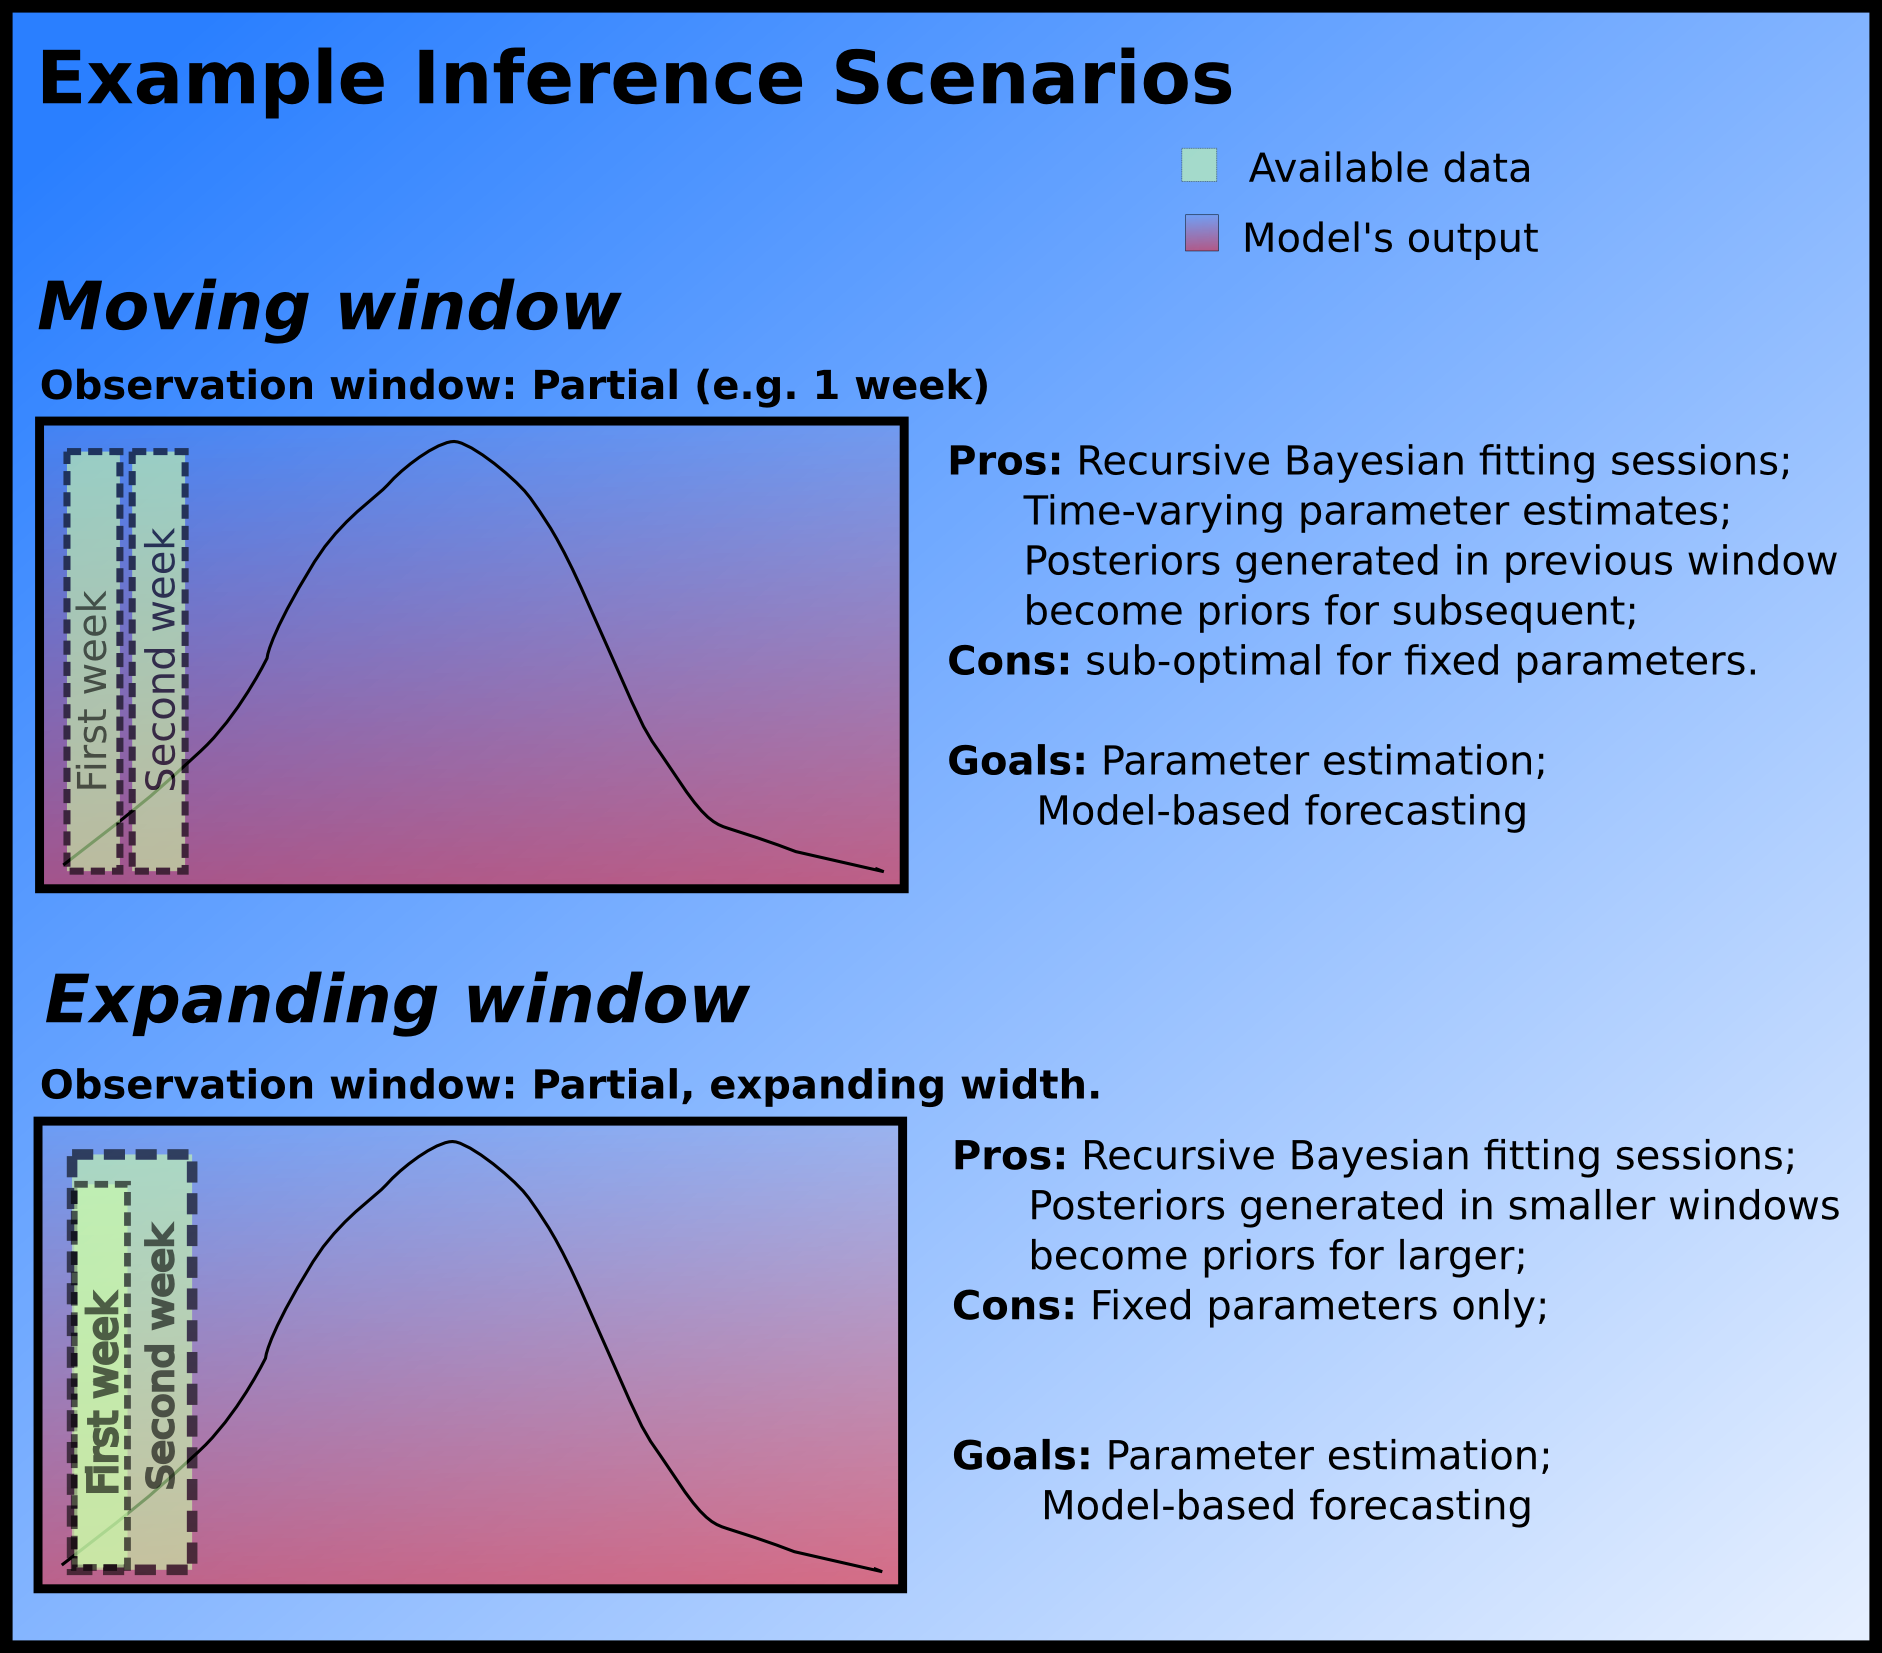
\includegraphics[width=15cm]{Inference_scenarios2.png}
\caption{Fitting scenarios: Moving windows and expanding windows.}\end{figure}


\subsection{References}

\resetcurrentobjects
\hypertarget{--doc-sde}{}

\hypertarget{sde}{}\section{Stochastic Differential Equations}

The SDE package in BIP, was born out of the need to simulate stochastic model to test the Parameters estimation routines in the Bayes Package. However, it is useful in many general-purpose application since it provides a pure Python implementation of an SDE solver.

Currently it provides a single solving algorithm, the Gillespie SSA. but other algorithms are planned for future releases


\chapter{Indices and tables}
\begin{itemize}
\item {} 
\emph{Index}

\item {} 
\emph{Module Index}

\item {} 
\emph{Search Page}

\end{itemize}


\renewcommand{\indexname}{Module Index}
\printmodindex
\renewcommand{\indexname}{Index}
\printindex
\end{document}
